\chapter{Introduction}\label{chap:intro}
\newcommand{\ignore}[1]{}
\ignore{Write this chapter LAST. Should be 5 to 10 pages. This chapter provides a quick summary of the
essential contents of the research project, principal results and contents of the report. The target
audience is members of the jury who do NOT have time to completely read all 21 reports, as well
academic members of other juries who wish to compare this work to other works.}

\section{Background}
\ignore{This is a generic title. Replace it with an actual title that describes the context of the work.
Short .5 page summary of the technological context of the work and why it is interesting or important}

3D animation can be a painstakingly tedious activity. To create a desired animation, animators go through the long process of keyframing. Keyframes are set positions that define the start and end points of a movement, sequences of poses which are transformed in time. Typically, animators assign poses to certain frames over time, so that in-between motions can be generated by a computer. To get an accurate animation, artists usually must assign many keyframes, then spend time adjusting and editing them to be more precise. The fact that industry professionals take so much time and effort to do this shows that for an amateur or untrained artist, creating \textit{good} 3D animation is close to impossible. 

In \autoref{fig:keyframes}, the highlighted object -- the ball flying through the window -- has keyframes attached to it on the timeline, which represent its various positions and rotations in time. Even in a simple bouncing ball animation like this one, relatively speaking, many keyframes are required: 20 keyframes for a simple object to move within seven seconds. I invite the reader to imagine the amount of keyframes an articulated character might require, considering each joint is its own object.

%\begin{wrapfigure}{R}{0.5\textwidth}
\begin{figure}[h!]
\centering
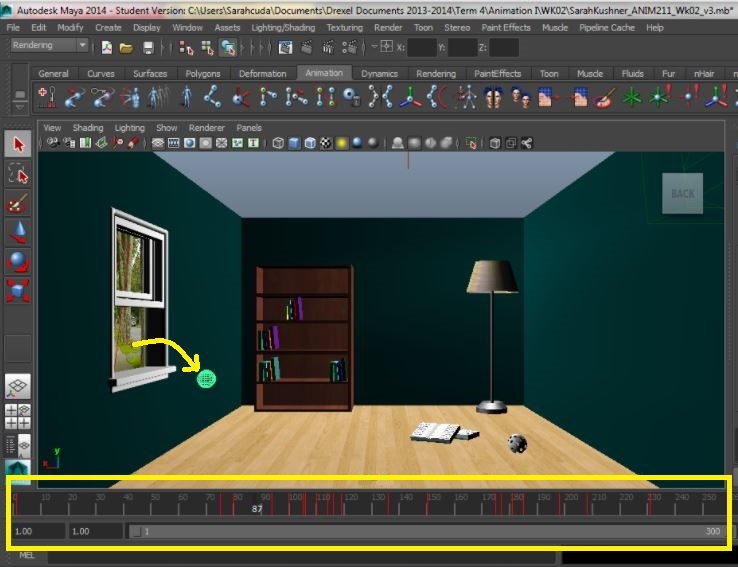
\includegraphics[scale=0.47]{img/keyframe}
\caption{Example of keyframing in Autodesk Maya. Each of the red lines on the timeline at the bottom indicate a keyframe for the highlighted object.}
\label{fig:keyframes}
\end{figure}
%\end{wrapfigure}

\section{Problem Statement}
\ignore{This is a generic title. Replace it with an actual title that describes the context of the work.
Approx .5 to 1 page description of the research problems that was addressed and what was required to address it.}

Among the most complicated characters to animate in 3D animation are humanoid characters. To ease this task, animators create a skeleton for their character called a rig, that consists of joints connected by bones to give a structure to the character. Humanoid rigs can range in complexity from (somewhat) simple to extremely complicated depending on the amount of detail desired by the user. The structure is a hierarchy of joints that can also be seen as a tree with a root, which in the humanoid case, is usually the pelvis. The leaf nodes of this tree, which are loacted at the maximal parts of the body, are the hands, feet, and head of the character. Leaf nodes come at the end of a kinematic chain, which can be followed back up to the root.


\begin{figure}[h!]
	\centering
        \begin{subfigure}[b]{0.55\textwidth}
        	\centering
                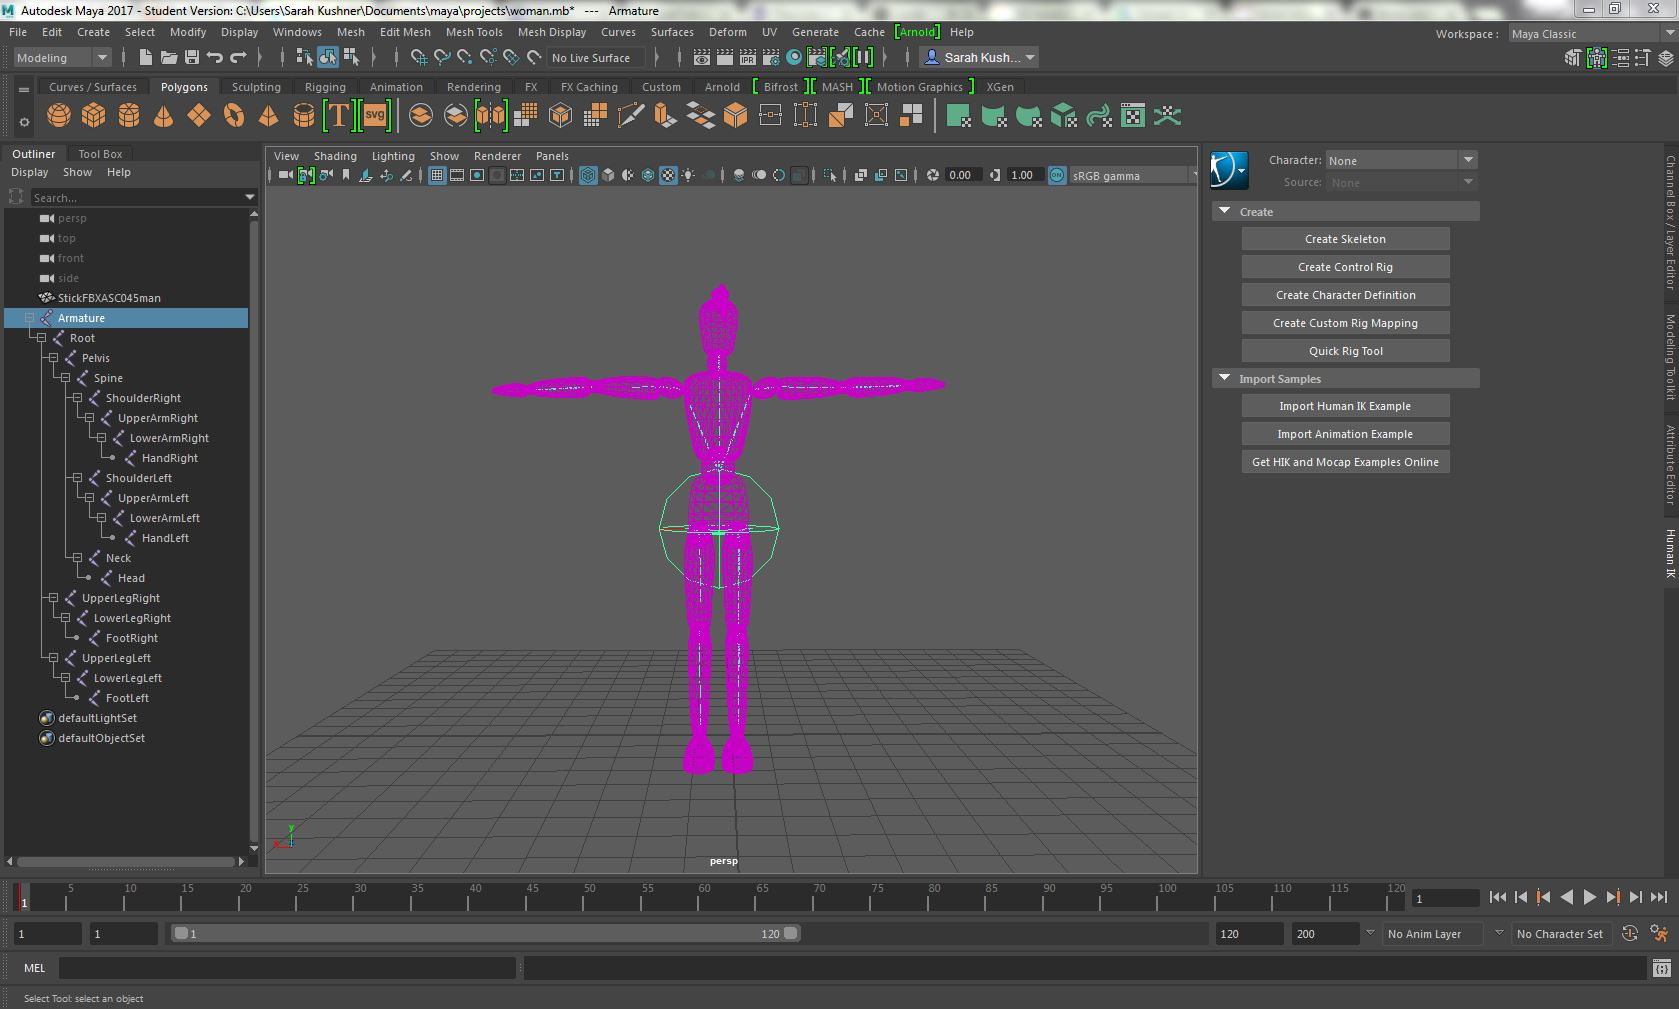
\includegraphics[width=\linewidth]{img/skeleton}
                \caption{Example of a humanoid skeleton.}
                \label{fig:skeleton}
        \end{subfigure}
        \quad
        \begin{subfigure}[b]{0.4\textwidth}
        	\centering
                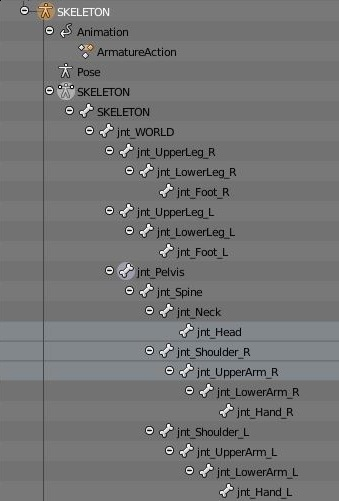
\includegraphics[width=\linewidth]{img/skeleton_hierarchy}
                \caption{The hierarchy of joints corresponding to the skeleton.}
                \label{fig:hierarchy}
        \end{subfigure}%
	\caption{Humanoid skeleton shown in Blender.}
	\label{fig:rig}
\end{figure}

\subsection{Kinematics}
Forward and inverse kinematics are two general animation methods used mainly in situations in which articulated characters need to move according to some contraints. In order to animate this structure successfully, controls are added that allow for forward and inverse kinematics. These controls help the animator move the character into poses that will then act as keyframes.

Forward kinematics (FK) is a method of calculating the position and orientation of the end of a kinematic chain (i.e. a hand or foot) given the positions and angles of the joints higher up in the chain all the way to the root. 

Inverse kinematics (IK) is the method opposite of forward kinematics. That is, the goal is to calculate the angles and positions of joints in the chain, given the angle and position of just the end of the chain. This goal is much harder to reach, seeing that more information needs to be calculated than is given. This problem is underconstrained. Many IK algorithms exist to calculate joint angles and positions, which will be discussed in \autoref{chap:theory}.

\subsection{Multiple Characters}
The animation of multiple characters, along with all the previously mentioned challenges, comes with its own unique set as well. The line of action technique works extremely well for a single humanoid character, and even multiple humanoid characters separate from each other. The problem is discovered when the humanoid characters interact, when they are in close proximity to each other or when they touch each other.

Occlusion and collisions can both become issues, especially when more than one character is involved.

\subsection{Posing}
posing

\section{Scientific Approach and Investigative Method and Results}
\ignore{This is a generic title. Replace it with an actual title that describes the context of the work.
Approx 1 to 2 page description of the scientific approach or approaches to a solution and how it was investigated and evaluated. Present a summary of the principal results obtained.}
The use case for this research in multi-character animation is a dancing couple. There are many combinations of poses a human can be in, let alone two humans \textit{and} the two humans interacting as one.

I traced dancers. traced keyframes. drew lines of action all over videos.

Found patterns.

Found common poses.

developed



\section{Contents of this report}
\ignore{Approx .5 page per chapter. Summarize the contents of the subsections of each chapter. Give the
topics addressed and summarize what is written in each chapter.}

In the following chapter (\autoref{chap:sota}), I cover the state-of-the-art for this particular problem. I discuss a brief history of dance notation -- how choreographers and dancers use sketching on paper to brainstorm and communicate their ideas of motion, formation, and pose of dance. Then I will talk about the existing sketch-based systems used for posing articulated characters, covering the benefits and limitations of each. A sizeable portion of my work has had to do with kinematic trees and graph data structures, so I will go into a few important graph theory algorithms. Generating animation from existing data is also a widely used technique relevant to my work.

In \autoref{chap:theory}, ...

